\documentclass[green]{GL2020}

\usepackage{array}
\usepackage{xcolor}
\usepackage{hyperref}
\usepackage{multicol}
\usepackage{ltablex}
\usepackage{tabularx}
\renewcommand{\tabularxcolumn}[1]{m{#1}}
\setlength{\columnsep}{1cm}

\usepackage{graphicx}
\graphicspath{ {C:/Users/charf/Documents/GitHub/GL2020/Puzzles/} }


\parindent=0pt
\begin{document}
\name{\gWeekendSchedule{}}

Below is the full event schedule, including both in game and out of game activities as of 14Oct2022. No IC events are mandatory for players to attend. They are probably good places to find other characters, or good times to sneak off and do something secret. The Pre-Game OOC events \textbf{are} mandatory, for the safety and coherence of the event. Post-game OOC events are optional. However, since these activities affect when carpools can leave, players should plan to be on site until 5 pm on Sunday, even if they personally wish to opt out of post game workshops.

Dinner on Friday is OOC, as it occurs before the game begins. Time to mingle and socialize as players is important for building rapport that facilitates intense play. Dinner on Saturday is also OOC, to give everyone a break. All other meals are optionally in character for soft RP, or OOC, as players choose. We will designate spaces for IC and OOC in the dining hall if it proves valuable.

This schedule is subject to change between now and game start as in and out of game needs mandate. We will have a final copy of the schedule at game, which will supersede this one if any changes are made.

%%%%%%%% Meal times: 8 am, 12 pm, 5:30 pm

For workshops on Friday afternoon, please pack a jacket and sunscreen in an easily accessible place, we will be outside the whole time, and you may want to grab one or both.

\begin{tabularx}{\textwidth}{|>{\centering\arraybackslash} m{1.6cm} | >{\centering\arraybackslash} m{1.6cm} | >{\centering\arraybackslash} m{1.8cm} | >{\centering\arraybackslash}X |}
 \hline
\multicolumn{4}{|c|}{\textbf{Friday (Mandatory Pre-Game Activities) 12:00 pm}} \\
\hline 
 \emph{Time} & \emph{Location} & \emph{Event} & \emph{Description}\\
\hline
 12:00 pm - 1:00 pm   & TBD & Registration &  Players will check in with the logistics team. Hard copies of game material will be provided. Either eat on the way to the venue, or bring food for a picnic lunch. \\
    \hline
  1:00 pm - 1:15 pm  & TBD & Workshop Orientation & Introduction to Workshops. The workshops are designed to help players get into character, create shared cultural touchpoints, and foster trust among players. \\
    \hline
  1:15 pm - 1:45 pm & TBD & Logistics Briefing & Logistics team will review camp and game policies with all players. \\
    \hline
  1:50 pm - 3:20 pm & TBD & Safety, Calibration, and Combat & Players will be split up across nation and cohort. This workshop will cover safety mechanics, how calibration and negotiation are used in this game, and practice the combat mechanic.\\
 \hline
  3:25 pm - 4:25 pm & TBD & Workshop by Country & Players will be split up by home nation. We will create a few cultural touchstones, reflect on social inequalities within the nation, and discuss the impacts of the war. \\
 \hline
  4:30 pm - 5:00 pm & TBD  &  Workshop by Cohort & Players will be split up by cohort. We will create a few social norms, reflect on the role of the cohort in the Time of Deciding, and consider the influence of magic on everyone's lives. We'll send you off with some questions to think about regarding your expectations for game.\\
 \hline
 5:00 pm - 5:30 pm & Sleeping Spaces  & Load-in & Time for players to unpack from cars into sleeping spaces. \\
 \hline
  5:30 pm - 6:30 pm & Dining Hall & Dinner. & Please eat food! This is also time to hang out and do any calibration you need to with other players you haven't had a chance to interact with before this point. If you need extra costuming time, feel free to leave dinner early. \\
 \hline
  6:30 pm - 7:00 pm & Sleeping Spaces  & Costuming & Time to get into costume, settle in, ask GMs last minute questions, and otherwise get ready for game. \\
 \hline
\multicolumn{4}{|c|}{\textbf{GAME ON 7:00 pm}} \\
\hline 
7:00 pm & Bobbitt Hall & Game Starts & \cPrincipal{\full} should have a few words to say to start the Time of Deciding. \\
 \hline
  8:30 pm - 8:45 pm & TBD  & First Storm Surge & Characters should probably take shelter in the bunkers. Traditionally characters shelter by country during this surge. \\
\hline
  10 pm & Everywhere & Quiet Hours Start & Quiet Hours start now. GM HQ closes for the night.\\
\hline
  12 am & Everywhere  & Game Off & Please get some sleep. \\
    \hline
 \end{tabularx}
  

\begin{tabularx}{\textwidth}{|>{\centering\arraybackslash} m{1.6cm} | >{\centering\arraybackslash} m{1.6cm} | >{\centering\arraybackslash} m{1.8cm} | >{\centering\arraybackslash}X |}
\hline
\multicolumn{4}{|c|}{\textbf{Saturday}} \\
 \hline
\emph{Time} & \emph{Location} & \emph{Event} & \emph{Description}\\
\hline
  8:00 am - 8:50 am & Dining Hall & Breakfast & Please eat food! This meal is optionally available for soft RP.  \\
\hline
  8:50 am - 9:00 am & Dining Hall & Game Announcements & GMs may have game related announcements (IC or OOC) at this time, so please plan to attend.  \\
\hline
\multicolumn{4}{|c|}{\textbf{GAME ON 9:00 am}} \\
\multicolumn{4}{|c|}{(Players are welcome to take time after official game start to put on costumes and makeup.)} \\
\hline 
  10:30 am - 11:00 am  & Bobbitt Hall & Ceremony of Excellence & \cMusic{\full} is in charge of organizing the Ceremony of Excellence to showcase the talent at the school. Characters are encouraged, but not mandated, to attend.  \\
 \hline
  12:00 pm - 1:00 pm & Dining Hall & Lunch & Please eat food! This meal is optionally available for soft RP. \\
 \hline
  2:00 pm - 2:15 pm & TBD & Second Storm Surge & Characters should probably take shelter in the bunkers. Traditionally characters shelter by job cohort during this surge. \\
\hline
  3:30 pm - 4:00 pm & Bobbitt Hall & Scientific Presentation & \cHeadScientist{\full} and \cAssistantScientist{\full} are scheduled to present the details of the ongoing research into ending the Storms for good.\\
\hline
 5:30 pm - 6:30 pm & Dining Hall & Dinner & Please eat food! This meal is \textbf{mandatorily OOC}. There will be an optional personal reflection and expectation management activity available for players to pursue individually.\\
\hline
 9 pm & TBD (GM HQ)  & Voting Authority mechanics due & Many players will need to submit information related to the mechanics for determining voting authority no later than 9 pm so GMs can tally it all up before morning.\\
\hline
  10 pm & Everywhere & Quiet Hours Start & Quiet Hours start now. GM HQ closes for the night.\\
\hline
  12 am & Everywhere & Game Off & Please get some sleep. \\
\hline
\end{tabularx}

\begin{tabularx}{\textwidth}{|>{\centering\arraybackslash} m{1.6cm} | >{\centering\arraybackslash} m{1.6cm} | >{\centering\arraybackslash} m{1.8cm} | >{\centering\arraybackslash}X |}
\hline
\multicolumn{4}{|c|}{\textbf{Sunday}} \\
\hline
\emph{Time} & \emph{Location} & \emph{Event} & \emph{Description}\\
\hline
8:00 am - 8:50 am & Dining Hall & Breakfast & Please eat food! This meal is optionally available for soft RP.  \\
\hline
8:50 am - 9:00 am & Dining Hall & Game Announcements & GMs may have game related announcements (IC or OOC) at this time, so please plan to attend.  \\
\hline
\multicolumn{4}{|c|}{\textbf{GAME ON 9:00 am}} \\
\multicolumn{4}{|c|}{(Players are welcome to take time after official game start to put on costumes and makeup.)} \\
\hline
10:00 am - 10:15 am  & TBD & Third Storm Surge & Characters should probably take shelter in the bunkers. There is no traditional grouping for this surge. \\
\hline
  11:30 am & Bobbitt Hall & Votes to Direct the Storm Due & Students must submit their votes for where to send the storm by this time. Uncast votes will be forfeit past this time so the GMs can tally the votes.\\
\hline
  12:00 pm - 1:00 pm & Dining Hall & Lunch & Please eat food! This meal is optionally available for soft RP.   \\
 \hline
  1:30 pm - 2:00 pm & Bobbitt Hall & Ritual To Control the Storm & The actual ritual to control where the storm is sent will happen at this time.\\
\hline
\multicolumn{4}{|c|}{\textbf{GAME ENDS 2:30 pm}} \\
\hline
\end{tabularx}

\begin{tabularx}{\textwidth}{|>{\centering\arraybackslash} m{1.6cm} | >{\centering\arraybackslash} m{1.6cm} | >{\centering\arraybackslash} m{1.8cm} | >{\centering\arraybackslash}X |}
\hline
\multicolumn{4}{|c|}{\textbf{Sunday (Optional Post-Game Activities) 2:30 pm}} \\
\hline
2:30 pm - 2:50 pm & TBD & Deroleing Exercise & Players may choose to join us for a guided activity to begin separating the player from the character and begin processing the weekend. Alternately, players may choose to help with tear down, or reflect alone.\\
 \hline
  2:50 - 4:00 pm & TBD & Game Wrap Up and Goodbyes & Players may choose to join us for a structured wrap-up for game. The GMs will sketch a few key epilogue pieces, and players will be able to share some of their character's story.\\
 \hline
  4:00 to 5:00 pm & Everywhere & Tear Down and Load Out & We will finish cleaning up and loading out from game! Once everyone in your carpool is packed out, cars may leave at any time, although the GMs would appreciate help cleaning up game too.  \\
 \hline
  5:00 pm & Everywhere & Event End & Drive safely on your way home! Everyone must be off-site by 5 pm.  \\
	\hline
\end{tabularx}
\clearpage

\center
{\LARGE Site Map}\\
\vspace{0.5cm}
\begingroup
\vfill
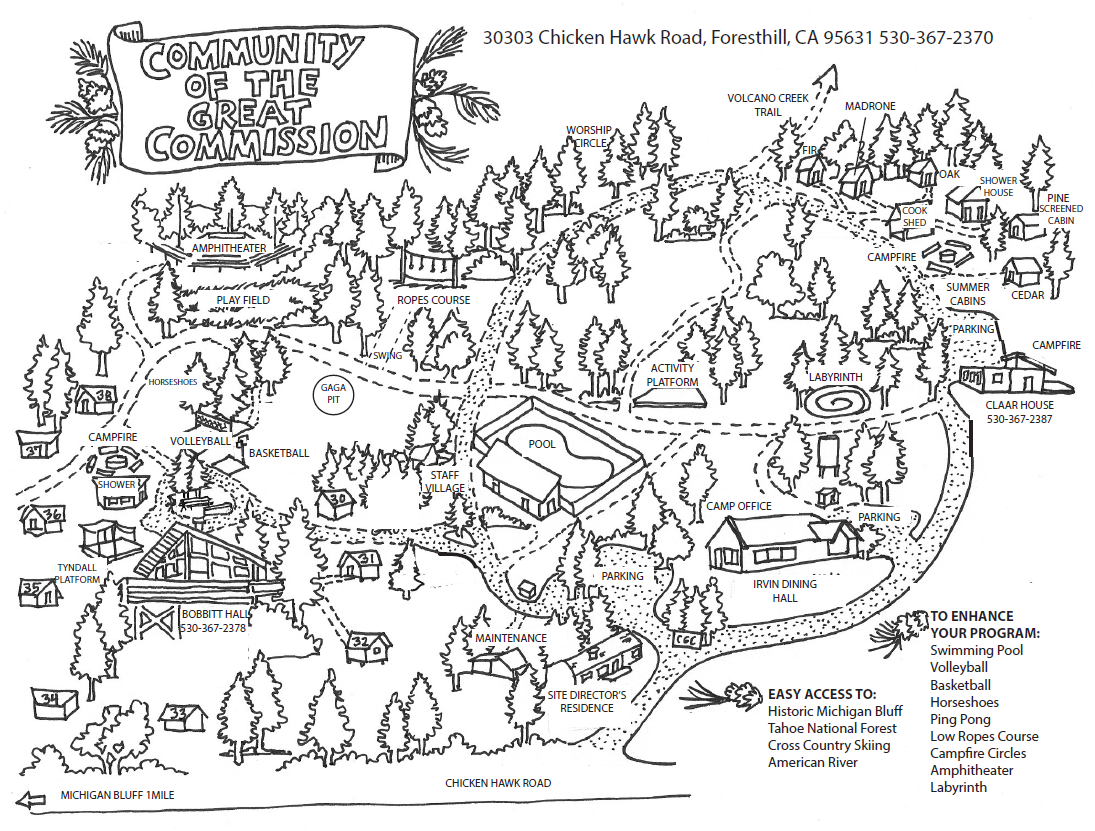
\includegraphics[angle=90,origin=c,scale=0.9]{SiteMap}
\vfill
\endgroup
\endcenter




\end{document}
